\documentclass[12pt]{article}
\usepackage[frenchb]{babel} 
\usepackage[T1]{fontenc}
\usepackage[utf8]{inputenc}
%\usepackage{lmodern} 
\usepackage{graphicx}
\usepackage{caption}
\usepackage{multirow}
\usepackage[top=2.5cm, bottom=2.5cm, left=2.5cm , right=2.5cm]{geometry}
%\usepackage{amsmath}
%\usepackage{amsthm}
%\usepackage{amsfonts}
\usepackage{empheq}
\usepackage{setspace}
\usepackage{hyperref}
\hypersetup{pdftitle = {ELE8812 - Rapport de laboratoire}, pdfauthor={Julien Antoine}}
\usepackage{color}
\usepackage{subfigure}
\usepackage{fancyvrb}
\usepackage{SIunits}
\usepackage{numprint}
\usepackage{enumitem}
\usepackage{calc}
\usepackage{listings}
\usepackage{float}
\usepackage{cellspace}
\cellspacetoplimit=4pt
\cellspacebottomlimit=4pt

% ----------------------------------- FANCY HEADER -----------------------------------
\usepackage{fancyhdr}
\pagestyle{fancy}
\renewcommand{\headrulewidth}{0.5pt}
%\fancyhead[C]{\textbf{page \thepage}} 
\fancyhead[L]{}
\fancyhead[R]{Rapport de laboratoire 3}

\renewcommand{\footrulewidth}{0.5pt}
\fancyfoot[C]{\textbf{\thepage}} 
\fancyfoot[L]{Polytechnique Montréal}
\fancyfoot[R]{ELE8812}
% ------------------------------------------------------------------------------------


\providecommand{\e}[1]{\ensuremath{\cdot 10^{#1}}}
\newcommand{\question}{\noindent$\bullet$\;\;}
\newcommand{\eau}{\ensuremath{\text{H}_2 \text{O}}}
\newcommand{\dio}{\ensuremath{\text{CO}_2}}
%\addto\captionsfrancais{\renewcommand{\chaptername}{Labo}}

\definecolor{mygreen}{RGB}{28,172,0} % color values Red, Green, Blue
\definecolor{mylilas}{RGB}{170,55,241}

\begin{document}

\lstset{language=Matlab,%
	%basicstyle=\color{red},
	breaklines=true,%
	morekeywords={matlab2tikz},
	keywordstyle=\color{blue},%
	morekeywords=[2]{1}, keywordstyle=[2]{\color{black}},
	identifierstyle=\color{black},%
	stringstyle=\color{mylilas},
	commentstyle=\color{mygreen},%
	showstringspaces=false,%without this there will be a symbol in the places where there is a space
	numbers=left,%
	numberstyle={\tiny \color{black}},% size of the numbers
	numbersep=9pt, % this defines how far the numbers are from the text
	emph=[1]{for,end,break},emphstyle=[1]\color{red}, %some words to emphasise
	%emph=[2]{word1,word2}, emphstyle=[2]{style},    
}

\hyphenation{HyperLogLog experimental techno-logy according develop-ment}

\begin{titlepage}
\newcommand{\HRule}{\rule{\linewidth}{0.5mm}} % Defines a new command for the horizontal lines, change thickness here

%-------------------------------------------------------------------------------------
%	LOGO SECTION
%-------------------------------------------------------------------------------------
\centering

\includegraphics[width = 0.33\textwidth]{../../logo}\\[5cm] 
\centering
%-------------------------------------------------------------------------------------
%	TITLE SECTION
%-------------------------------------------------------------------------------------
\HRule \\[0.4cm]
{ \huge \bfseries ELE8812 -- Rapport de laboratoire 5}\\[0.4cm] 
{ \Large \bfseries Compression d'images}\\
\HRule \\[1cm]
%-------------------------------------------------------------------------------------
%	AUTHOR SECTION
%-------------------------------------------------------------------------------------
\begin{minipage}{0.45\textwidth}
\begin{center} 
\large
Julien \textsc{Antoine}\\
1813026
\end{center}
\end{minipage}
~
\begin{minipage}{0.45\textwidth}
\begin{center} 
\large
Maxime \textsc{Schmitt}\\
1719088
\end{center}
\end{minipage}\\[8cm]
%-------------------------------------------------------------------------------------
%	DATE SECTION
%-------------------------------------------------------------------------------------
\begin{center}
{\Large 6 avril 2016}
\end{center}
%-------------------------------------------------------------------------------------
\vfill 
\end{titlepage}

%\tableofcontents

\section{Introduction}



\section{Test du codeur/décodeur}
\subsection{Image \textsf{cameraman.tif}}
Appliquons premièrement la compression EPEG sur l'image \textsf{cameraman.tif}. La figure \autoref{subfig:cameraImg} montre l'image originale, et le résultat des compressions EPEG et JPEG. On observe que la compression EPEG dégrade beaucoup plus l'image que JPEG pour un même taux de compression. 
La figure \autoref{subfig:cameraErr} permet d'observer l'erreur quadratique des deux normes, avant et après avoir été zippées. On observe que pour JPEG, l'erreur augmente exponentiellement avec le taux de compression, ce qui parait normal puisqu'en compressant on élimine de l'information, et donc de la qualité et des détails. On remarque que le fait de zipper l'image compressée ne change pas l'erreur quadratique, du moins pas de manière visible. 

Pour EPEG, le résultat est complètement différent: on distingue que la courbe possède un puits, dans lequel l'erreur est minimale. Cela s'explique assez simplement: la matrice de quantification qui divise les coefficients de la transformée en cosinus discrète est multipliée par le coefficient de compression $\alpha$. Dès lors, lorsque ce dernier est trop grand, la quantification est très destructive (beaucoup de coefficients deviennent nuls), et lorsqu'il est trop faible, les coefficients deviennent supérieurs (en valeur absolue) à 127 et le contraste est diminué. Ce phénomène s'observe d'ailleurs très bien sur la figure \autoref{subfig:cameraImg}. Il existe donc une valeur optimale du coefficient de compression pour laquelle l'erreur est minimale. On note également qu'après zippage, le taux de compression est augmenté sans influencer l'erreur quadratique (cela s'exprime par le décalage de la courbe vers la gauche), ce qui signifie que la norme EPEG est moins efficace que JPEG, pour qui la compression zip supplémentaire est rendue inutile.

\begin{figure}[!h] 
	\centering
	\subfigure[Effet sur l'image]{
		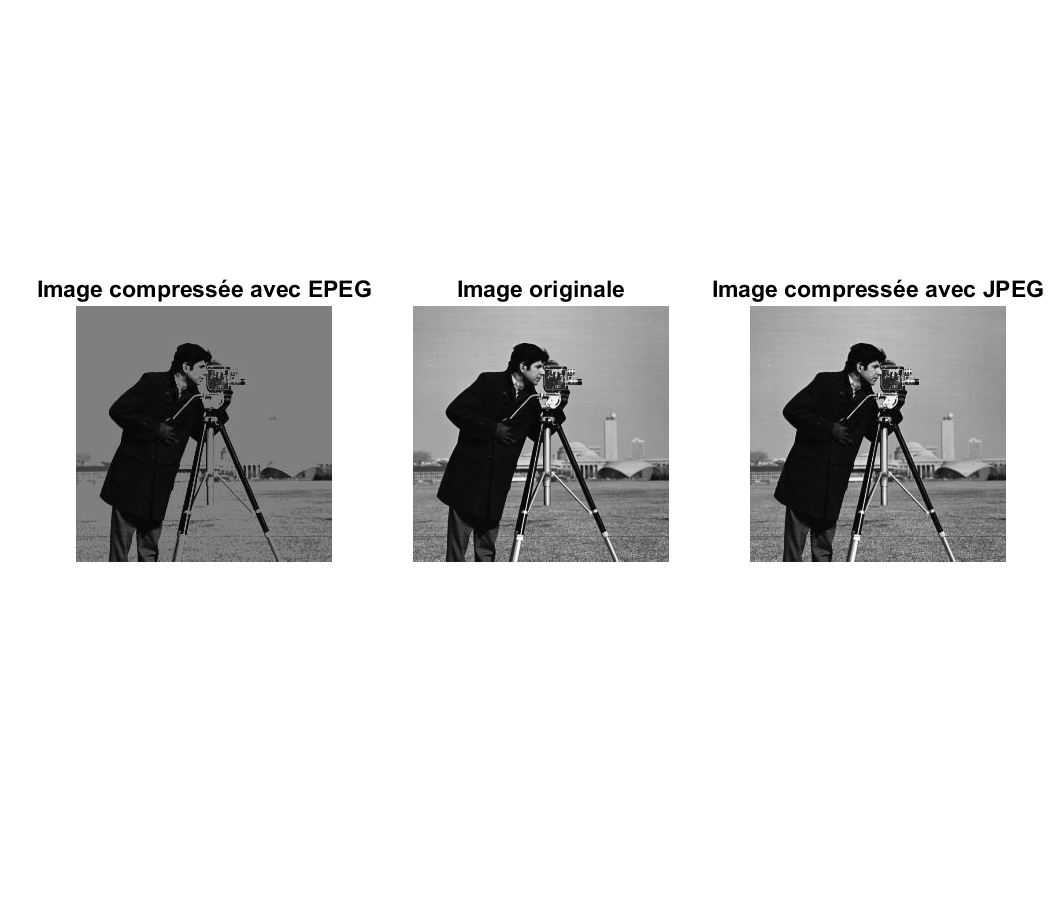
\includegraphics[width = 0.46\textwidth]{images/cameramanEPEGComparaison}
		\label{subfig:cameraImg} }
	\quad
	\subfigure[Erreur quadratique]{
		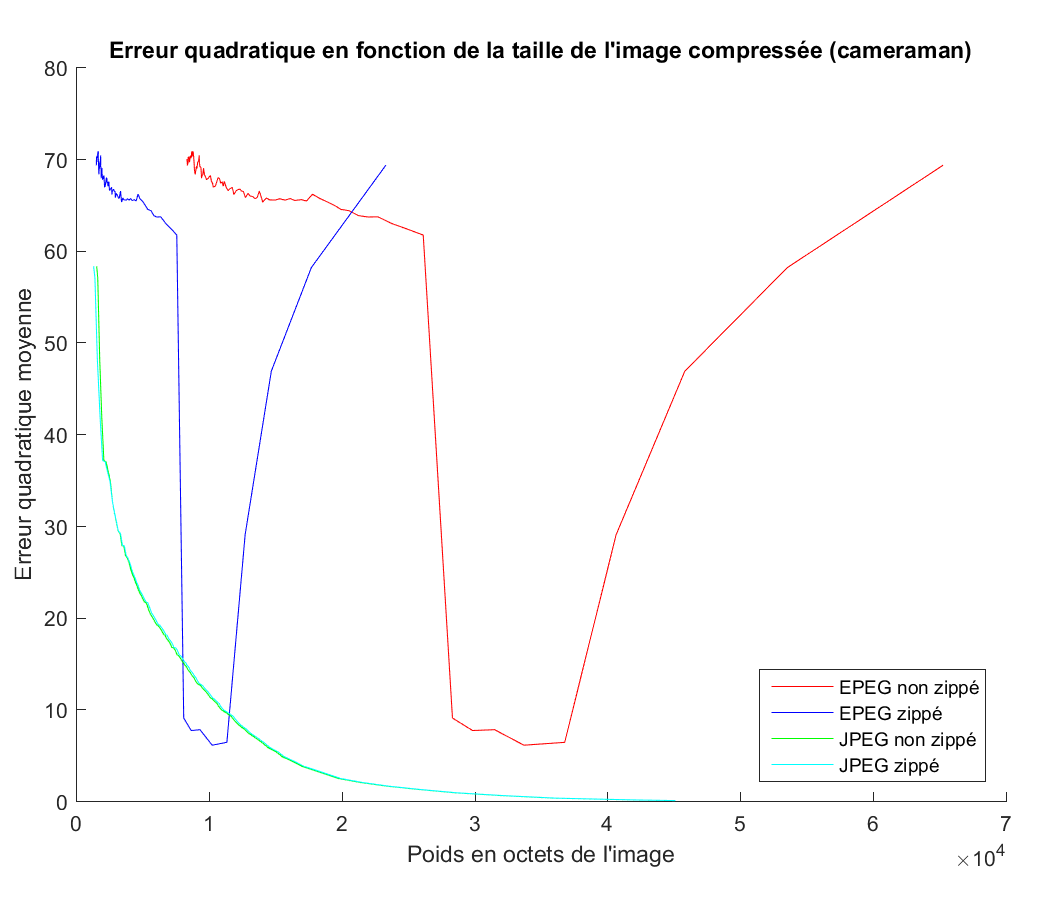
\includegraphics[width = 0.46\textwidth]{images/quadraticErrorCameraman}
		\label{subfig:cameraErr} }
	\caption{Compression de l'image \textsf{cameraman.tif}} 
	\label{fig:cameraman}
\end{figure}


\subsection{Image \textsf{paolina.tif}}
La figure \autoref{fig:paolina} permet de faire le même constat pour l'image \textsf{paolina.tif}. JPEG est toujours plus efficace que EPEG, qui contient un puits semblable mais plus large que pour l'image \textsf{camerman.tif}. Comme précédemment, le fait de zipper n'influence pas l'erreur après une compression JPEG, tandis que cela améliore la compression EPEG. On observe encore une diminution flagrante du contraste en utilisant EPEG, contrairement à JPEG.


\begin{figure}[!h] 
	\centering
	\subfigure[Effet sur l'image]{
		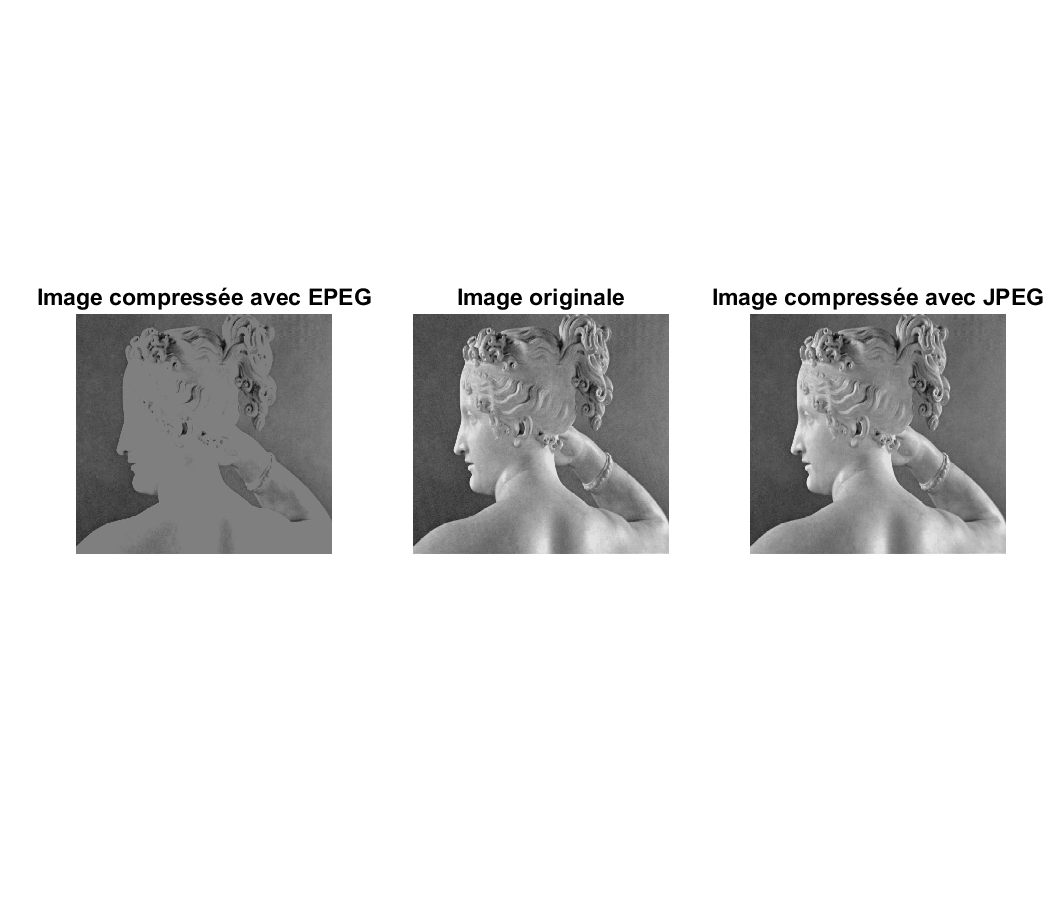
\includegraphics[width = 0.46\textwidth]{images/paolinaEPEGComparaison}
		\label{subfig:paolinaImg} }
	\quad
	\subfigure[Erreur quadratique]{
		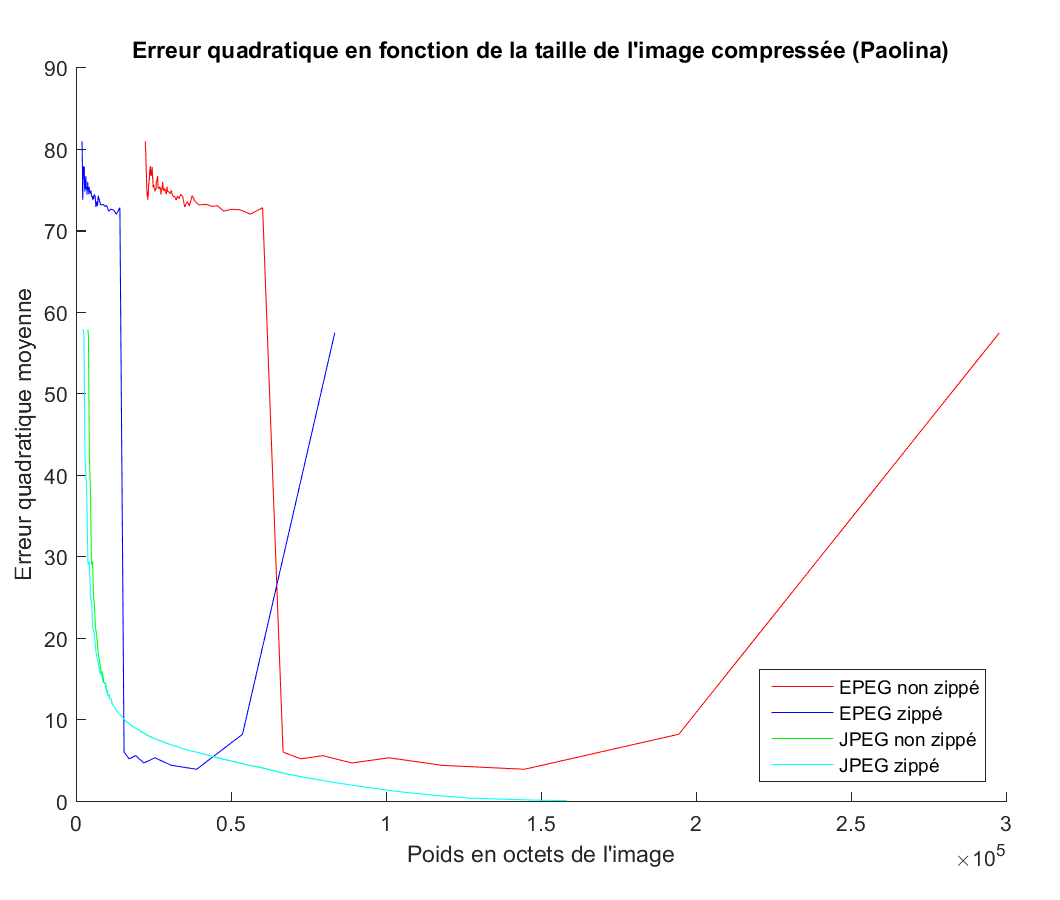
\includegraphics[width = 0.46\textwidth]{images/quadraticErrorPaolina}
		\label{subfig:paolinaErr} }
	\caption{Compression de l'image \textsf{cameraman.tif}} 
	\label{fig:paolina}
\end{figure}






%\newpage
%\section*{Annexe A - Code partie : .m}
%\label{annexe3}
%\lstinputlisting{../src/ex3.m}

\end{document}